% !TEX root = ../my-thesis.tex
%
\chapter{Data Analysis}
\label{sec:analysis}
In this chapter the models fitted for each country are reviewed. First, a look at the standardised incidence rate for each country is taken, before spatial models, spatio-temporal models and finally predictive models are discussed.
\section{Standardised Incidence Ratio (SIR)}
This section takes a brief look at the SIR for the countries of interest. Recall from Equation~\ref{eq:sir}, that the SIR is defined as the ratio of observed counts to expected counts.
\subsection{SIR for Germany}
When looking at the SIR for Germany in Figure~\ref{sirgermany}, it is noticeable that the actual number of infections in the eastern parts of Germany, especially in Saxony, is considerably higher than the expected number of infections. Furthermore, parts of Bavaria have an increased SIR compared to the rest of Germany, excluding Saxony. This could be due to the fact that the regions share a border with the Czech Republic, a country that is substantially more affected by Covid-19 than Germany. The northern parts of Germany show the lowest SIR which is possibly due to the fact that this region is sparsely populated.
% \begin{figure}[H]
%   \centering
%   \includesvg[width = 1.2\textwidth]{sir_germany.svg}
%   \caption{The SIR for Germany based on the data of the 24th of March 2021}
%   \label{sirgermany}
% \end{figure}
\begin{figure}[H]
  \centering
  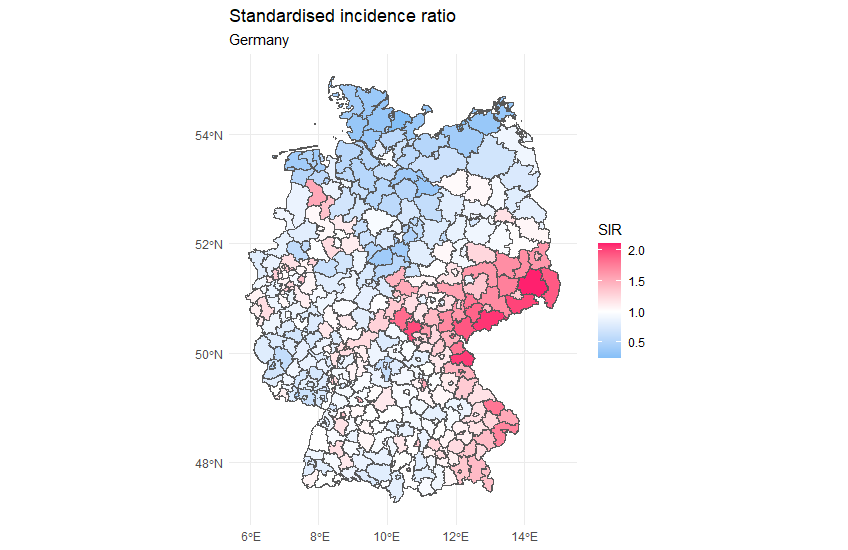
\includegraphics[width = 1.2\textwidth]{sir_germany.png}
  \caption{The SIR for Germany based on the data of the 24th of March 2021}
  \label{sirgermany}
\end{figure}
\subsection{SIR for Norway}
Looking at the standardised incidence rate for Norway in Figure~\ref{sirnorway}, a standardised incidence rate of less than 1 can be seen for most municipalities north of Trondheim. In the southern parts of Norway there are several municipalities with a rate above 1, for example the standardised incidence rate around the capital Oslo is around 2. However, the two small municipalities, Hyllestad and Ulvik, have the highest standardised incidence rate in Norway. In Hyllestad, 95 of 1328 people have been infected with Covid-19 so far, while in Ulvik, 134 of 1080 people have been infected so far. \\
The SIR in Hyllestad is around 4.5, following an outbreak in a shipyard in autumn 2020 \cite{newspaper1}, while Ulvik has a ratio of around 8, following an outbreak of the UK variant of Covid-19. According to the head of the municipality, Hans Petter Thorbjørnsen, the infections are thought to have spread through children \cite{newspaper2}.
% \begin{figure}[H]
%   \centering
%   \includesvg[width = 1.2\textwidth]{sir_norway.svg}
%   \caption{The SIR for Norway based on the data of the 24th of March 2021}
%   \label{sirnorway}
% \end{figure}
\begin{figure}[H]
  \centering
  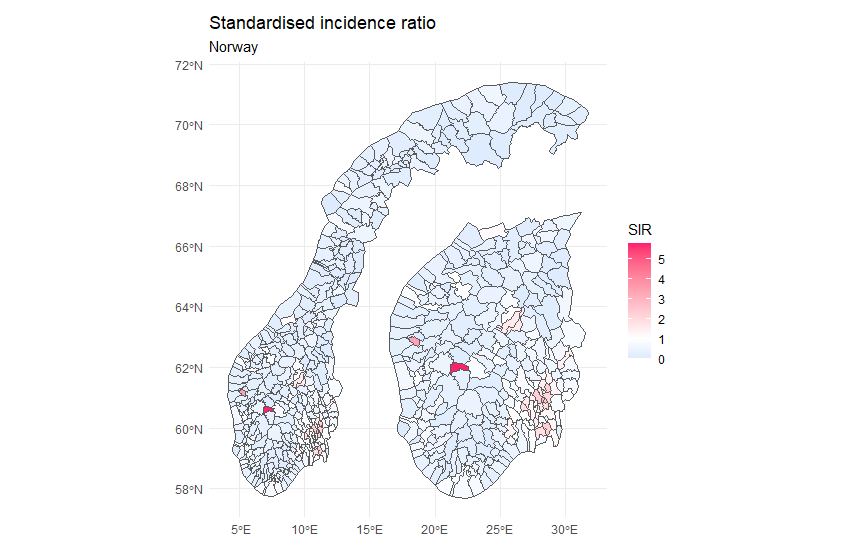
\includegraphics[width = 1.2\textwidth]{sir_norway.png}
  \caption{The SIR for Norway based on the data of the 24th of March 2021}
  \label{sirnorway}
\end{figure}
Because the high numbers from two small municipalities complicate the interpretation of Figure~\ref{sirnorway}, Figure~\ref{sirnorwaylog} shows the SIR on a log10 scale. On this scale, a value of 0 means that the risk of infection in a given municipality is neither lower nor higher. Values below 0 mean that the risk of infection in a municipality is lower than average, while values above 1 mean that the risk of infection in a municipality is higher than average. It is now clearer that the standardized incidence ratio is below 1 in most parts of Norway, but that there is a higher risk in the region around Oslo.
% \begin{figure}[H]
%   \centering
%   \includesvg[width = 1.2\textwidth]{sir_norway_log.svg}
%   \caption{The log10 SIR for Norway based on the data of the 24th of March 2021}
%   \label{sirnorway}
% \end{figure}
\begin{figure}[H]
  \centering
  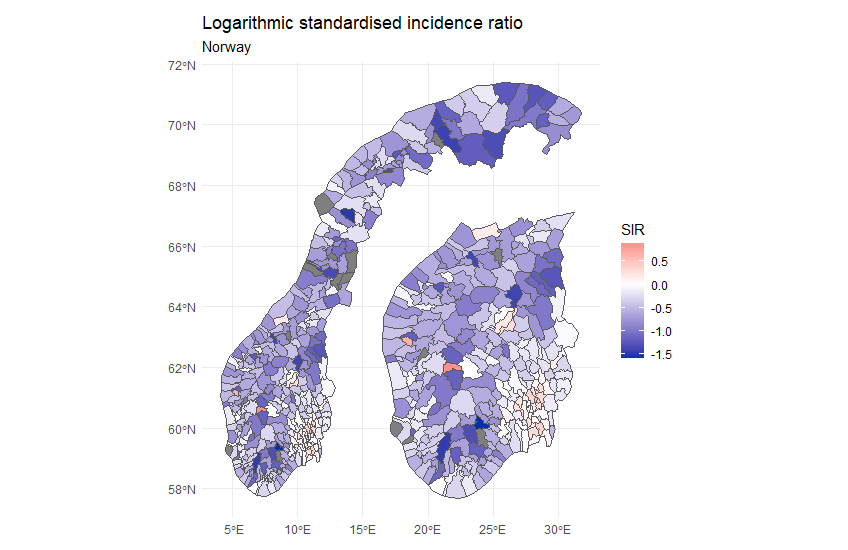
\includegraphics[width = 1.2\textwidth]{sir_norway_log.png}
  \caption{The log10 SIR for Norway based on the data of the 24th of March 2021}
  \label{sirnorwaylog}
\end{figure}
\clearpage
\section{Data Modelling}
After looking at the standardised incidence rates for the countries of interest, the next step is to take a closer look at the current figures for the respective countries. Spatial models are used to try to extract the factors that cause some populations to be at higher risk than populations in other geographical regions. Three different types of models are used for each country:
\begin{itemize}
    \item[1.] Besags Proper Spatial Model
    \item[2.] A Leroux Model
    \item[3.] A BYM2 Model
\end{itemize}
All of these models are computed using the INLA \cite{rinla} R package. \\
To specify each type of model, the code shown in Listing~\ref{codeModels} can be used. \\
The measures introduced in Section~\ref{sec:performance}, namely the DIC, the WAIC, the CPO and the mean absolute error (MAE), are used to compare the models.\\
For all countries, the models are computed with
\begin{itemize}
    \item[1.] only the demographic variables as covariates
    \item[2.] only the infrastructural variables as covariates
    \item[3.] both, demographic and infrastructural variables, as covariates
\end{itemize}
In addition to specifying what type of spatial model to use, if any, there is also the option of specifying a prior. \\
As can be seen in Section~\ref{sec:pc_prior}, a pc prior can be specified for the precision parameter $\tau$, which is what is done here. \\
For the parameters $\sigma_0$ and $\alpha$ in Equation~\ref{eq:pc_prior_prec} the values 1 and 0.01 are chosen. \\
The models are compared using the mean absolute error. For this, 20\% of the observations are removed from the training set and used for testing instead. The predicted number of infections for these municipalities is then compared to the actual numbers.
\\
% Finally, due to the amount of covariates, forwards and backwards stepwise variable selection was performed with the intention of obtaining a model that fits the data well and at the same time is relatively easy to interpret. This can be done with the R package \texttt{INLAutils} \cite{inlautils}, as shown in Listing~\ref{codeSelection}. Backwards as well forwards variable selection was performed.\\
A list of all calculated models along with their performance measures is provided in the appendix.
\subsection{Choice of Likelihood}
Before the models are computed, however, the distribution that fits the number of cases must first be found. One way to do this, the function \texttt{descdist()} from the \texttt{fitdistrplus} R package is used. The Cullen and Frey graph illustrates how "close" a sample is to a theoretical distribution based on the kurtosis and the square of the skewness, defined in Equation~\ref{eq:kurtosis} and Equation~\ref{eq:skewness}. It can be used to get a preliminary idea of which distributions fit the data, in this case the number of infections, reasonably well. \\
The plots for Germany and Norway can be seen in Figure~\ref{cf_germany} and Figure~\ref{cf_norge}. The blue dot represents the data, the star a theoretical normal distribution, the dashed line a theoretical Poisson distribution and the grey area a theoretical negative binomial distribution. In both cases, the blue dot is relatively far from the star and lies in the region of a negative binomial distribution. For the Norwegian sample shown in Figure~\ref{cf_norge}, the sample is closer to a Poisson distribution than is the case for the German sample in Figure~\ref{cf_germany}.
% \begin{figure}[H]
%     \centering
%     \includesvg[width = 0.8\textwidth]{cf_germany.svg}
%     \caption{The Cullen and Frey graph for Germany}
%     \label{cf_germany}
% \end{figure}
\begin{figure}[H]
    \centering
    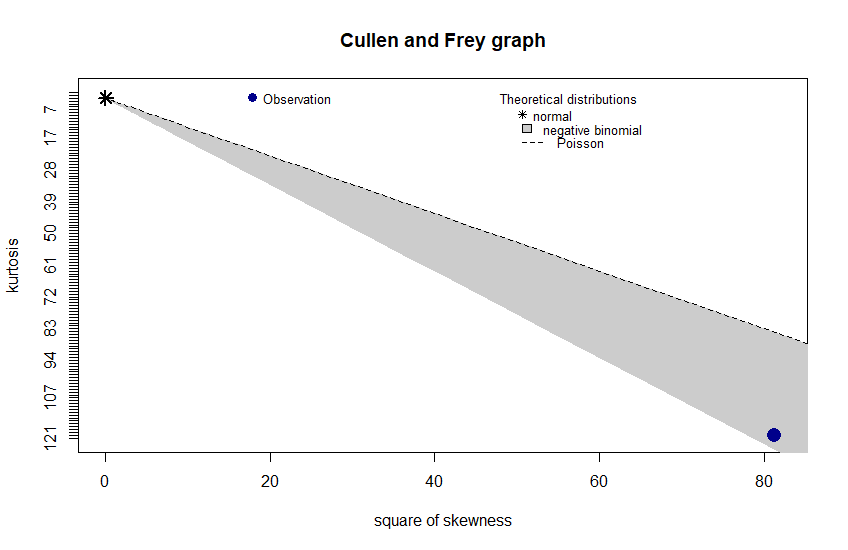
\includegraphics[width = 0.8\textwidth]{cf_germany.png}
    \caption{The Cullen and Frey graph for Germany}
    \label{cf_germany}
\end{figure}
% \begin{figure}[H]
%     \centering
%     \includesvg[width = 0.8\textwidth]{cf_norge.svg}
%     \caption{The Cullen and Frey graph for Norway}
%     \label{cf_norge}
% \end{figure}
\begin{figure}[H]
    \centering
    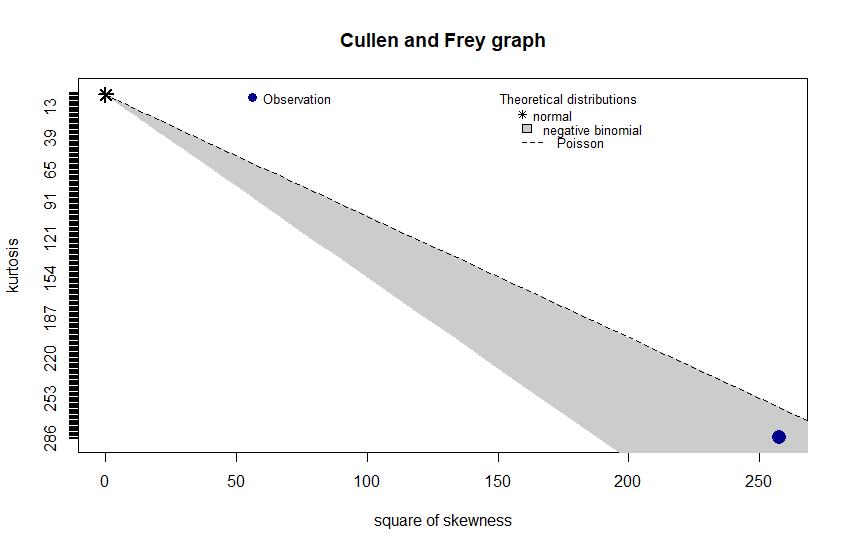
\includegraphics[width = 0.8\textwidth]{cf_norge.png}
    \caption{The Cullen and Frey graph for Norway}
    \label{cf_norge}
\end{figure}
Next, a negative binomial distribution, a normal distribution, and a Poisson distribution are fitted to the data using the maximum likelihood method. The negative binomial fits for both countries can be seen in Figure~\ref{fitNegbinomGermany} and Figure~\ref{fitNegbinomNorway}. The fits for the normal and Poisson distribution for both countries, are shown in the Appendix in Figure~\ref{fitNormalGermany}, Figure~\ref{fitPoissonGermany}, Figure~\ref{fitNormalNorway} and Figure~\ref{fitPoissonNorway}. \\
The QQ-plot for Germany and Norway looks quite similar, as there appears to be a linear relationship between the theoretical quantile and the sample quantiles, up to a certain point where the sample quantiles have a higher value than the theoretical quantiles, indicating that the distribution is right skewed. Since there are many municipalities with relatively few cases and few municipalities with a large number of cases, this is to be expected. It can also be seen that the empirical cumulative density function closely follows the theoretical cumulative density function.
% \begin{figure}[H]
%     \centering
%     \includesvg[width = 0.8\textwidth]{fit_nbinom_germany.svg}
%     \caption{A negative binomial fit to the number of cases in German municipalities}
%     \label{fitNegbinomGermany}
% \end{figure}
\begin{figure}[H]
    \centering
    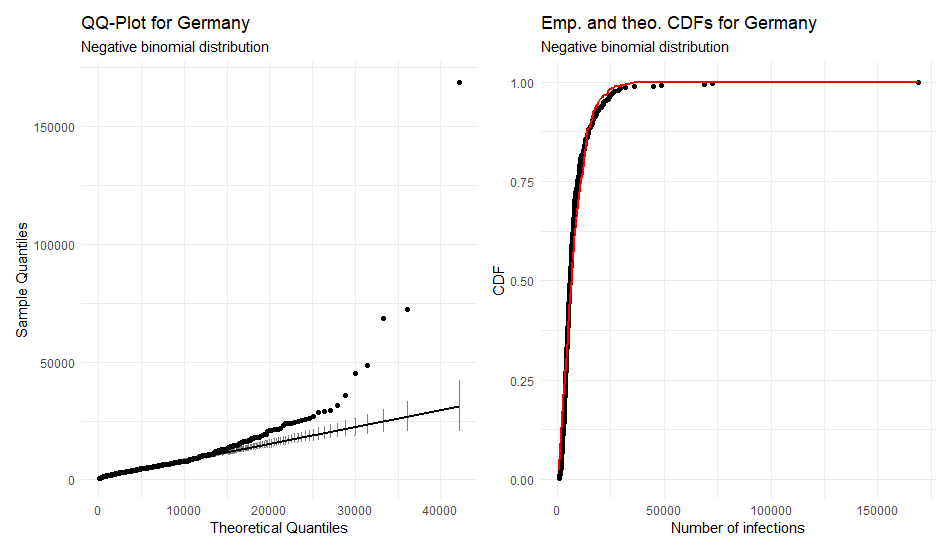
\includegraphics[width = 0.8\textwidth]{fit_nbinom_germany.png}
    \caption{A negative binomial fit to the number of cases in German municipalities}
    \label{fitNegbinomGermany}
\end{figure}
% \begin{figure}[H]
%     \centering
%     \includesvg[width = 0.8\textwidth]{fit_nbinom_norway.svg}
%     \caption{A negative binomial fit to the number of cases in Norwegian municipalities}
%     \label{fitNegbinomNorway}
% \end{figure}
\begin{figure}[H]
    \centering
    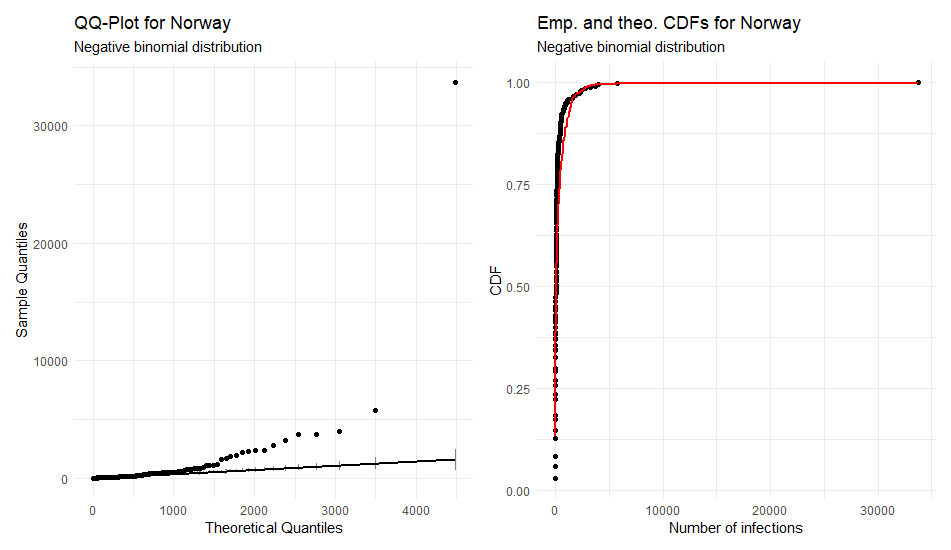
\includegraphics[width = 0.8\textwidth]{fit_nbinom_norway.png}
    \caption{A negative binomial fit to the number of cases in Norwegian municipalities}
    \label{fitNegbinomNorway}
\end{figure}
Lastly, the AIC is calculated for fitting a normal distribution to the data, a Poisson distribution to the data and a negative binomial distribution to the data. The values can be seen in Table~\ref{aic}. Afterwards, the negative binomial distribution is chosen as the distribution of the target variable in both cases. \\
\begin{table}[H] 
\caption{The AIC for different distributions for Germany and Norway \label{aic}}
\begin{tabular}{l l r}
\toprule
\textbf{Country}	& \textbf{Distribution}	& \textbf{AIC} \\
\midrule
Germany & Normal & 8360 \\
Germany & Poisson & 2148100 \\
Germany & Negative Binomial & 7731 \\
Norway & Normal & 6166 \\
Norway & Poisson & 366181 \\
Norway & Negative Binomial & 4086 \\
\bottomrule
\end{tabular}
\end{table} 
The poor fit for the Poisson distribution can be explained by looking at the range of the number of confirmed cases in a given municipality. For Germany, this number ranges from 508 to 137634 (as of March 18, 2021), while for Norway, the number ranges from 0 to 24905 (as of March 20, 2021). This results in a mean and standard deviation for Germany of 6617 and 9014, respectively. For Norway, the values for these metrics are 236 and 1389. This is problematic because, as shown in Equation~\ref{eq:poisson_exp} and Equation~\ref{eq:poisson_var}, for a Poisson distribution the expected value and the variance should be equal. \\
Looking at a histogram for the confirmed number of cases and overlaying the densities of a normal, Poisson and a negative binomial distribution helps to confirm the choice of a negative binomial distribution as the distribution that the data most closely resembles. Figure~\ref{fitDistrGermany} and Figure~\ref{fitDistrNorway} both show that a negative binomial distribution fits the data better than a normal distribution. Due to the high values for the AIC, the Poisson distribution is excluded from these graphics.
% \begin{figure}[H]
%     \centering
%     \includesvg[width = 0.8\textwidth]{distrfit_germany.svg}
%     \caption{Histogram for the number of cases in German municipalities with a normal and a negative binomial distribution overlayed..}
%     \label{fitDistrGermany}
% \end{figure}
\begin{figure}[H]
    \centering
    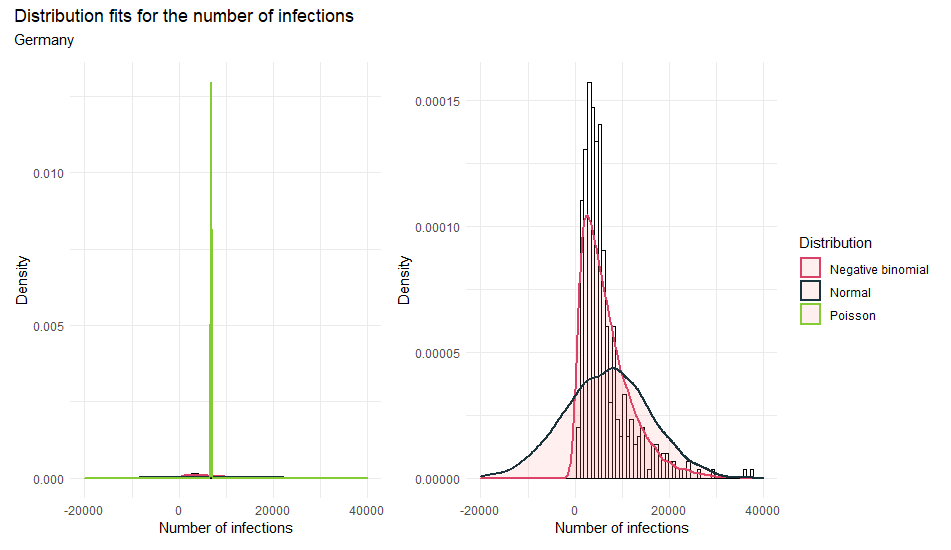
\includegraphics[width = 0.8\textwidth]{distrfit_germany.png}    
    \caption{Histogram for the number of cases in German municipalities with a normal and a negative binomial distribution overlayed.}
    \label{fitDistrGermany}
\end{figure}
% \begin{figure}[H]
%     \centering
%     \includesvg[width = 0.8\textwidth]{distrfit_norway.svg}    
%\caption{Histogram for the number of cases in Norwegian municipalities with a normal and a negative binomial distribution overlayed.}
%     \label{fitDistrNorway}
% \end{figure}
\begin{figure}[H]
    \centering
    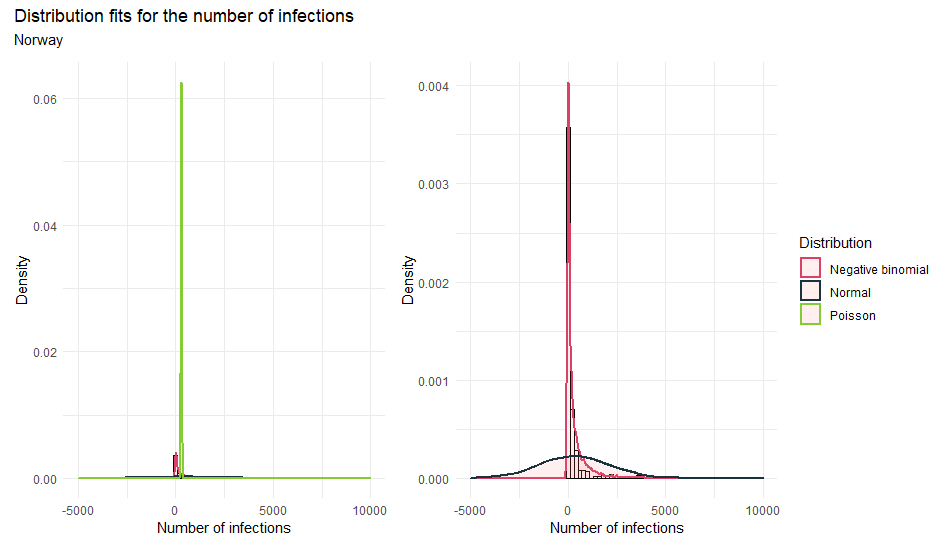
\includegraphics[width = 0.8\textwidth]{distrfit_norway.png}
    \caption{Histogram for the number of cases in Norwegian municipalities with a normal and a negative binomial distribution overlayed.}
    \label{fitDistrNorway}
\end{figure}
\clearpage
\section{Models without a Spatial Component}\label{sec:nospatial}
To establish a baseline, a look is first taken at models that do not include a spatial effect. This way, it can be observed how the means and credibility intervals of the covariates change when a spatial effect is added to a model and how the performance of the model changes with respect to the goodness-of-fit indicators introduced in Section~\ref{sec:performance}. \\
Before computing the models, using the $\hbox{VIF}$ introduced in Section~\ref{sec:vif}, predictors are removed if their $\hbox{VIF}$ is above 5. To do this, an OLS regression is first run on all variables, followed by the calculation of $\hbox{VIF}$. Then the variable with the highest value is removed before running the regression model again with all remaining variables. This process is repeated until only variables with a $\hbox{VIF}$ of less than 5 remain. \\
In sections~\ref{sec:nospatial_germany} and~\ref{sec:nospatial_norway} the results of these models are presented. Their goodness-of-fit indicators as well as the coefficients together with their credibility intervals calculated as in section~\ref{sec:mean_iv} are reported. \\
These models are based on data from 24 March 2021, when 2,695,037 people were infected with Covid-19 in Germany, while 87,537 people were infected in Norway. The five municipalities with the most infections in Germany are shown in Table~\ref{top5germany} and in Table~\ref{top5norway} for Norway.
\begin{table}[H] 
\caption{The German municipalities with the most infections as of March 24th 2021. \label{top5germany}}
\begin{tabular}{l r r}
\toprule
\textbf{Municipality}	& \textbf{Population}	& \textbf{Number of infections} \\
\midrule
SK Berlin & 3644826 & 141639   \\     
SK Hamburg & 1841179 & 58661   \\
SK Munich & 1471508 & 57690   \\
SK Cologne & 1085664 & 37592   \\
Region Hannover & 1157624 & 36241   \\
\bottomrule
\end{tabular}
\end{table}
\begin{table}[H] 
\caption{The Norwegian municipalities with the most infections as of March 24th 2021. \label{top5norway}}
\begin{tabular}{l r r}
\toprule
\textbf{Municipality}	& \textbf{Population}	& \textbf{Number of infections} \\
\midrule
Oslo & 693494 & 26151 \\
Bergen & 283929 & 4738 \\
Drammen & 101386 & 3149 \\
Bærum & 127731 & 2834 \\
Lillestrøm & 85983 & 2779 \\
\bottomrule
\end{tabular}
\end{table}
\subsection{Models without a Spatial Component for Germany}\label{sec:nospatial_germany}
Table~\ref{allGermany_nospatial} contains the performance measures for the baseline model for Germany, while Table~\ref{FixedAllGermany_nospatial} contains the posterior mean, the exponentiated posterior mean and the credibility intervals of the coefficients. It can be seen that the intercept as well as six of the coefficients are significant.
\begin{table}[H] 
\caption{The performance measures for the model without a spatial component. \label{allGermany_nospatial}}
\begin{tabular}{r r r r}
\toprule
\textbf{DIC}	& \textbf{WAIC} & \textbf{CPO} & \textbf{MAE}\\
\midrule
5504 & 5506 & -2778 &  179234 \\
\bottomrule
\end{tabular}
\end{table}
\begin{table}[H]
\caption{The fixed effects for the model. Values are rounded. A $^*$ denotes a significant effect. \label{FixedAllGermany_nospatial}}
\begin{tabular}{l r r r r c}
\toprule
\textbf{Variable}	& \textbf{mean$_{\hbox{p}}$}	& \textbf{exp(mean$_{\hbox{p}}$)} & \textbf{exp(q0025$_{\hbox{p}}$)} & \textbf{exp(q0975$_{\hbox{p}}$)} & \textbf{sig.}\\
\midrule
(Intercept) & -0.07213 & 0.9553 & 0.9291 & 0.9821 & $^*$\\
pop\_dens & 0.1566 & 1.170 & 1.115 & 1.227 & $^*$\\
log & \multirow{2}{*}{0.08821} & \multirow{2}{*}{1.093} & \multirow{2}{*}{1.041} & \multirow{2}{*}{1.146} & \multirow{2}{*}{$^*$}\\
trade\_tax \\
sex & 0.04363 & 1.045 & 1.009 & 1.081 & $^*$\\
platform & 0.03324 & 1.034 & 0.9796 & 1.091 \\
FDP & 0.03242 & 1.033 & 0.9945 & 1.073 \\
higher\_ & \multirow{2}{*}{0.01918} & \multirow{2}{*}{1.020} & \multirow{2}{*}{0.9787} & \multirow{2}{*}{1.063} \\
education\\
clinic & 0.01448 & 1.015 & 0.9608 & 1.073 \\
urb\_dens & 0.009294 & 1.010 & 0.9699 & 1.051 \\
aerodrome & -0.0009688 & 0.9991 & 0.9731 & 1.028 \\
nursing\_ & \multirow{2}{*}{-0.006835} & \multirow{2}{*}{0.9933} & \multirow{2}{*}{0.9609} & \multirow{2}{*}{1.027} \\
home\\
place\_of\_ & \multirow{2}{*}{-0.03459} & \multirow{2}{*}{0.9662} & \multirow{2}{*}{0.9256} & \multirow{2}{*}{1.008} \\
worship\\
marketplace & -0.03482 & 0.9663 & 0.9080 & 1.027 \\
office & -0.04362 & 0.9576 & 0.9140 & 1.004 \\
die\_linke & -0.0721 & 0.9306 & 0.8948 & 0.9676 & $^*$\\
SPD & -0.1316 & 0.8768 & 0.8476 & 0.9068 & $^*$\\
Gruene & -0.2816 & 0.7548 & 0.7197 & 0.7913 & $^*$\\
\bottomrule
\end{tabular}
\end{table}
\subsection{Models without a Spatial Component for Norway}\label{sec:nospatial_norway}
Table~\ref{allNorway_nospatial} contains the performance measures for the baseline model for Germany, while Table~\ref{fixedAllNorway_nospatial} contains the posterior mean, the exponentiated posterior mean and the credibility intervals of the coefficients. It can be seen that the intercept as well as five of the coefficients are significant.
\begin{table}[H] 
\caption{The performance measures for the model without a spatial component. \label{allNorway_nospatial}}
\begin{tabular}{r r r r}
\toprule\textbf{DIC}	& \textbf{WAIC} & \textbf{CPO} & \textbf{MAE}\\
\midrule
2713 & 2718 & -1623 & 10170 \\
\bottomrule
\end{tabular}
\end{table} 
\begin{table}[H]
\caption{The fixed effects for the model. Values are rounded. A $^*$ denotes a significant effect. \label{fixedAllNorway_nospatial}}
\begin{tabular}{l r r r r c}
\toprule
\textbf{Variable}	& \textbf{mean$_{\hbox{p}}$}	& \textbf{exp(mean$_{\hbox{p}}$)} & \textbf{exp(q0025$_{\hbox{p}}$)} & \textbf{exp(q0975$_{\hbox{p}}$)} & \textbf{sig.}\\
\midrule
(Intercept) & -0.8721 & 0.4185 & 0.3832 & 0.4569 & $^*$ \\
immigrants\_ & \multirow{2}{*}{0.2773}& \multirow{2}{*}{1.322}& \multirow{2}{*}{1.165}& \multirow{2}{*}{1.497}& \multirow{2}{*}{$^*$}\\
total \\
unemp\_ & \multirow{2}{*}{0.2086} & \multirow{2}{*}{1.236} & \multirow{2}{*}{1.062} & \multirow{2}{*}{1.435} & \multirow{2}{*}{$^*$} \\
immg\\
urb\_dens & 0.1790 & 1.200 & 1.027 & 1.423 & $^*$ \\
unemp\_tot & 0.07675 & 1.085 & 0.8969 & 1.304 \\
platform & 0.07141 & 1.078 & 0.9139 & 1.271 \\
higher\_ & \multirow{2}{*}{0.01850}& \multirow{2}{*}{1.020}& \multirow{2}{*}{0.9375}& \multirow{2}{*}{1.125}\\ 
education \\
nursing\_ & \multirow{2}{*}{0.01501} & \multirow{2}{*}{1.016} & \multirow{2}{*}{0.9377} & \multirow{2}{*}{1.117} \\
home\\
median\_age & -0.004360  & 0.9969 & 0.9020 & 1.098 \\
marketplace & -0.006536 & 0.9959 & 0.8735 & 1.145 \\
place\_of\_ & \multirow{2}{*}{-0.04057}& \multirow{2}{*}{0.9634}& \multirow{2}{*}{0.8233}& \multirow{2}{*}{1.130} \\
worship \\
office & -0.1372 & 0.8749 & 0.7434 & 1.030 \\
sex & -0.1535 & 0.8591 & 0.7691 & 0.9568 & $^*$ \\
aerodrome & -0.1954 & 0.8247 & 0.7010 & 0.9335 & $^*$ \\
\bottomrule
\end{tabular}
\end{table}
\clearpage
\section{Spatial Models}\label{ch:spatial}
Under the null hypothesis of no spatial autocorrelation, a p-value greater than 0.05 would be expected. The results of the test are presented in Table~\ref{moranTest}. Looking at the p-value for both countries, it can be seen that there is a spatial correlation for the number of infections in a municpality.
\begin{table}[H] 
\caption{Results of the Moran test for Germany and Norway. \label{moranTest}}
\begin{tabular}{l r r r r}
\toprule
\textbf{Country} & \textbf{Moran's I}	& \textbf{$\mathbb{E}\left[I\right]$}	& \textbf{p-Value} \\
\midrule
Germany & 0.1047 & -0.002500 & < 0.01 \\
Norway & 0.1085 & -0.002817 & < 0.01 \\
\bottomrule
\end{tabular}
\end{table}
Therefore, after the models without spatial effect have been calculated and established as baseline models, a spatial term is added to the models calculated in Section~\ref{sec:nospatial} , in order to model this spatial correlation.
\subsection{Spatial Models for Germany}
Looking at the performance of the spatial models and the model with the spatial component shown in Table~\ref{allGermany}, it can be seen that the spatial models perform better in terms of the DIC, WAIC and MAE, while they perform equally well or better in terms of the CPO. \\
The best performance of all models, in terms of MAE, was observed for the BYM2 model, which slightly outperformed the Besag model.
\begin{table}[H] 
\caption{The performance measures for the best performing demographic + infrastructure model of each type. \label{allGermany}}
\begin{tabular}{l r r r r}
\toprule
\textbf{Model}	& \textbf{DIC}	& \textbf{WAIC} & \textbf{CPO} & \textbf{MAE}\\
\midrule
No spatial & 5504 & 5506 & -2778 & 179234 \\
Besag&  4706 & 4685 & -2738 & 176201\\
BYM2 & 4628 & 4612 & -2729 & 176017\\
Leroux & 5118 & 5108 & -2998 & 179150 \\
\bottomrule
\end{tabular}
\end{table}
Figure~\ref{intervalGermany} shows the differences between the coefficients in the model without the spatial component and the BYM2 model. Excluding the intercept, only three effects are significant in the BYM2 model compared to six in the model without the spatial component. Moreover, the coefficients of the BYM2 model are closer to 1 and have smaller credibility intervals. The reason for this is that when using a spatial field in combination with a PC prior, higher values for $\sigma_0$ make the spatial field larger, which in turn causes the posterior mean to shrink towards 1.
\begin{figure}[H]
    \centering
    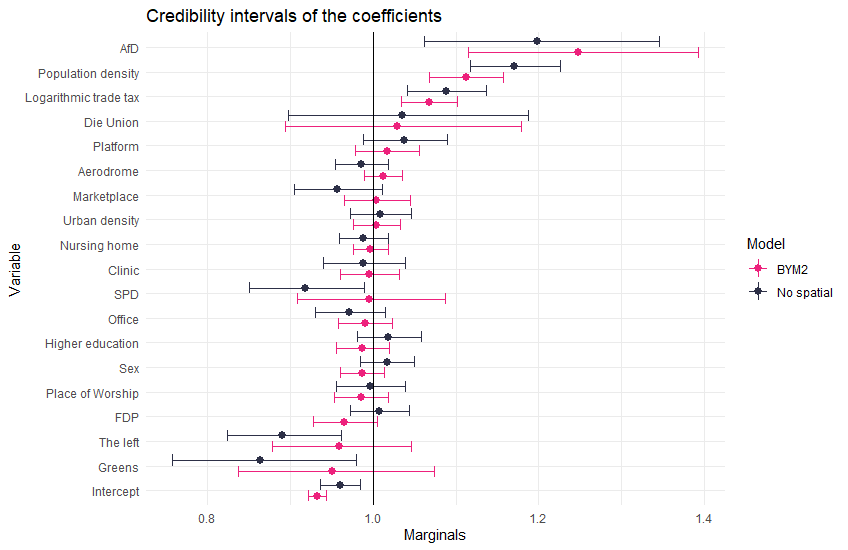
\includegraphics[width = \textwidth]{intervals_germany.png}
    \caption{The posterior mean and credibility intervals of the coefficients}
    \label{intervalGermany}
\end{figure}
% \begin{figure}[H]
%     \centering
%     \includesvg[width = textwidth]{intervals_germany.svg}
%    \caption{The posterior mean and credibility intervals of the coefficients}
%     \label{intervalGermany}
% \end{figure}
The values of the coefficients and credibility intervals are shown in Table~\ref{FixedAllGermany_spatial}.
\begin{table}[H]
\caption{The fixed effects for the model. Values are rounded. A $^*$ denotes a significant effect. \label{FixedAllGermany_spatial}}
\begin{tabular}{l r r r r c}
\toprule
\textbf{Variable}	& \textbf{mean$_{\hbox{p}}$}	& \textbf{exp(mean$_{\hbox{p}}$)} & \textbf{exp(q0025$_{\hbox{p}}$)} & \textbf{exp(q0975$_{\hbox{p}}$)} & \textbf{sig.}\\
\midrule
(Intercept) & -0.08087 & 0.9223 & 0.9105 & 0.9345 & $^*$\\
pop\_dens & 0.1084 & 1.115 & 1.066 & 1.165 & $^*$\\
log & \multirow{2}{*}{0.5714} & \multirow{2}{*}{1.059} & \multirow{2}{*}{1.022} & \multirow{2}{*}{1.097} & \multirow{2}{*}{$^*$}\\
trade\_tax \\
platform & 0.01315 & 1.013 & 0.9705 & 1.058 \\
die\_linke & 0.01160 & 1.012 & 0.9605 & 1.066 \\
marketplace & 0.01117 & 1.011 & 0.9669 & 1.057 \\
aerodrome & 0.009694 & 1.010 & 0.9919 & 1.028 \\
urb\_dens & 0.007543 & 1.008 & 0.9760 & 1.040 \\
sex & 0.004908 & 1.005 & 0.9746 & 1.036 \\
clinic & 0.004868 & 1.005 & 0.9648 & 1.047 \\
nursing\_ & \multirow{2}{*}{0.003748} & \multirow{2}{*}{1.004} & \multirow{2}{*}{0.9799} & \multirow{2}{*}{1.028} \\
home\\
FDP & -0.006087 & 0.9942 & 0.9507 & 1.039 \\
place\_of\_ & \multirow{2}{*}{-0.01738} & \multirow{2}{*}{0.9829} & \multirow{2}{*}{0.9483} & \multirow{2}{*}{1.018} \\
worship\\
office & -0.02228 & 0.9781 & 0.9428 & 1.014 \\
SPD & -0.02744 & 0.9732 & 0.9290 & 1.019 \\
higher\_ & \multirow{2}{*}{-0.02879} & \multirow{2}{*}{0.9718} & \multirow{2}{*}{0.9368} & \multirow{2}{*}{1.008} \\
education\\
Gruene & -0.1735 & 0.8410 & 0.7980 & 0.8856 & $^*$\\
\bottomrule
\end{tabular}
\end{table}
For the hyperparameters, a value of 14.22 is reported for the precision and a value of 0.9172 for $\phi$. Hence, 91.72\% of the marginal variance is explained by the structured effect. Therefore, this model is far from reducing to pure overdispersion and comes close to a Besag model, which is also reflected in the similar values of the goodness-of-fit indicators in Table~\ref{allGermany}.
\subsection{Spatial Models for Norway}
Comparing the performance of the models, the spatial models again showed better performance in terms of DIC and WAIC and this time also significantly better in terms of CPO. However, the model without the spatial component showed better predictive performance, as indicated by the lowest value for the MAE in Table~\ref{allNorway}. This could indicate that neighbourhood effects are not as strong in Norway as in Germany.
\begin{table}[H] 
\caption{The performance measures for the best performing demographic + infrastructure model of each type. \label{allNorway}}
\begin{tabular}{l r r r r}
\toprule
\textbf{Model}	& \textbf{DIC}	& \textbf{WAIC} & \textbf{CPO} & \textbf{MAE} \\
\midrule
No spatial & 2713 & 2718 & -1623 & 10170 \\
Besag  & 2452 & 2468 & -3782 & 11266 \\
BYM2 & 2278 & 2265 & -5627 & 11520\\
Leroux &  2272 & 2230 & -8261 & 11434\\
\bottomrule
\end{tabular}
\end{table}
Looking at the differences between the coefficients and credibility intervals in Figure~\ref{intervalNorway}, the picture is similar to Figure~\ref{intervalGermany}. In the BYM2 model, fewer effects are significant, two compared to five in the model without the spatial component, the coefficients are closer to 1 and the credibility intervals are narrower.
\begin{figure}[H]
    \centering
    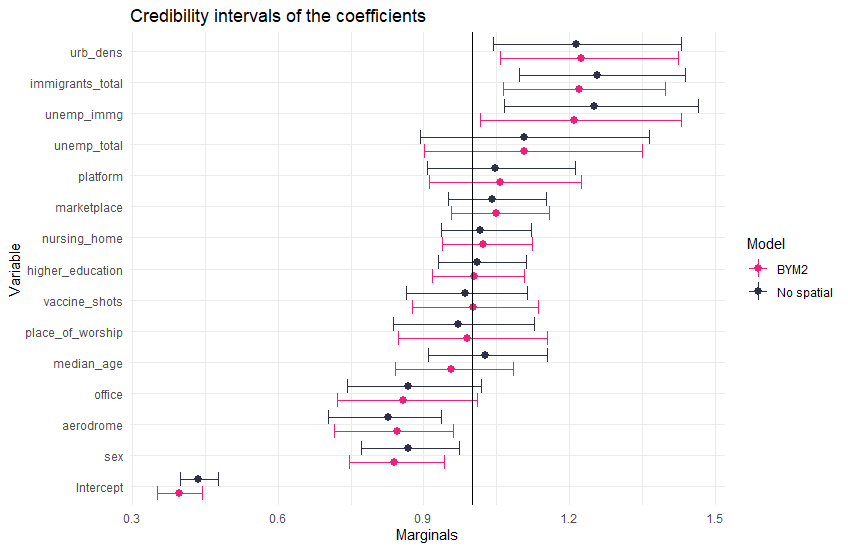
\includegraphics[width = \textwidth]{intervals_norway.png}
    \caption{The posterior mean and credibility intervals of the coefficients}
    \label{intervalNorway}
\end{figure}
% \begin{figure}[H]
%     \centering
%     \includesvg[width = textwidth]{intervals_norway.svg}
%    \caption{The posterior mean and credibility intervals of the coefficients}
%     \label{intervalNorway}
% \end{figure}
The values of the coefficients and credibility intervals are shown in Table~\ref{fixedAllNorway_spatial}.
\begin{table}[H]
\caption{The fixed effects for the model. Values are rounded. A $^*$ denotes a significant effect. \label{fixedAllNorway_spatial}}
\begin{tabular}{l r r r r c}
\toprule
\textbf{Variable}	& \textbf{mean$_{\hbox{p}}$}	& \textbf{exp(mean$_{\hbox{p}}$)} & \textbf{exp(q0025$_{\hbox{p}}$)} & \textbf{exp(q0975$_{\hbox{p}}$)} & \textbf{sig.}\\
\midrule
(Intercept) & -1.121 & 0.3260 & 0.3026 & 0.3504 & $^*$ \\
immigrants\_ & \multirow{2}{*}{0.1432} & \multirow{2}{*}{1.156} & \multirow{2}{*}{1.029} & \multirow{2}{*}{1.294} & \multirow{2}{*}{$^*$} \\
total \\
unemp\_tot & 0.08298 & 1.090 & 0.9203 & 1.281 \\
place\_of\_ & \multirow{2}{*}{0.08127} & \multirow{2}{*}{1.087} & \multirow{2}{*}{0.9488} & \multirow{2}{*}{1.242} \\
worship \\
unemp\_immg & 0.06734 & 1.073 & 0.9247 & 1.237 & \\
urb\_dens & 0.04398 & 1.047 & 0.9284 & 1.178 \\
marketplace & 0.01543 & 1.017 & 0.9041 & 1.142 \\
nursing\_ & \multirow{2}{*}{0.008396} & \multirow{2}{*}{1.009} & \multirow{2}{*}{0.9340} & \multirow{2}{*}{1.089} \\
home \\
higher\_ & \multirow{2}{*}{0.005382} & \multirow{2}{*}{1.006} & \multirow{2}{*}{0.9325} & \multirow{2}{*}{1.083} \\
education\\
sex & 0.004273 & 1.006 & 0.9073 & 1.112\\
platform & -0.02252 & 0.9805 & 0.8450 & 1.131 \\
office & -0.06488 & 0.9402 & 0.8004 & 1.095 \\
aerodrome & -0.09666 & 0.9097 & 0.7926 & 1.015 \\
median\_age & -0.1151  & 0.8925 & 0.8052 & 0.9853 & $^*$ \\
\bottomrule
\end{tabular}
\end{table}
\clearpage
For the hyperparameters, a value of 1.733 is reported for the precision and a value of 0.6249 for $\phi$. Hence, 62.49\% of the marginal variance is explained by the structured effect. Therefore, this model lies somewhere between pure overdispersion and the Besag model, but closer to the Besag model than to overdispersion.
\clearpage
\section{Choice of Hyperpriors}
As can be seen in Equation~\ref{pcprec}, there is flexibility when it comes to choosing the values for the standard deviation $\sigma_0$ as well as the probability $\alpha$. Therefore, an upper bound for the standard deviation can be chosen as well as the weight placed on this "tail event", describing how informative the resulting prior is. \\
Some of the issues that come with the choice of these hyperpriors were already discussed in Section~\ref{sec:issues}. \\
In the following, an assessment is made of how the performance of a Besag model, a BYM2 model and a Leroux model changes when playing around with the value for the standard deviation $\sigma_0$. To create these plots, models were calculated with $\sigma_0$ values of $\pmb{\sigma_0}=\left(0.1,0.11,0.12,...,5\right)$. Focus is only on the WAIC, as it is the only truly Bayesian performance measure, and the MAE to assess how the predictive performance changes.\\
In Figure~\ref{comparison_norway_1} it can be seen that when choosing a higher value for $\sigma_0$, the WAIC is lower in the case of the Besag model and the BYM2 model. For the Leroux model, on the other hand, the WAIC gets lower until about 2 before it rises until $\sigma_0 = 2.5$ and then falls again. It is a positive sign that this is not the case with the BYM2 model, as it was designed to avoid exactly this kind of thing. \\
For the MAE in Figure~\ref{comparison_norway_2}, it can be seen for both the BYM2 and the Besag model that a higher value for $\sigma_0$ leads to a higher value for the MAE. The same is true for the Leroux model, but again there is a small interval where it continuously decreases even though the value for $\sigma_0$ increases.
\begin{figure}[H]
    \centering
    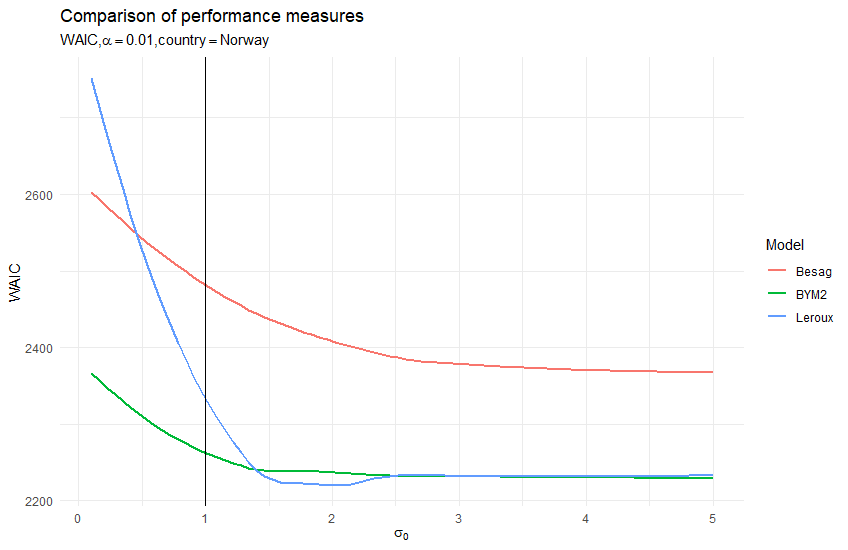
\includegraphics[width = \textwidth]{waic_norway_smooth.png}
    \caption{Value of the WAIC when changing the value for $\sigma_0$. The black line highlights the values for $\sigma_0$ = 1.}
    \label{comparison_norway_1}
\end{figure}
% \begin{figure}[H]
%     \centering
%     \includesvg[width = \textwidth]{waic_norway_smooth.svg}
%     \caption{Value of the WAIC when changing the value for $\sigma_0$. The black line highlights the values for $\sigma_0$ = 1.}
%     \label{comparison_norway_1}
% \end{figure}
\begin{figure}[H]
    \centering
    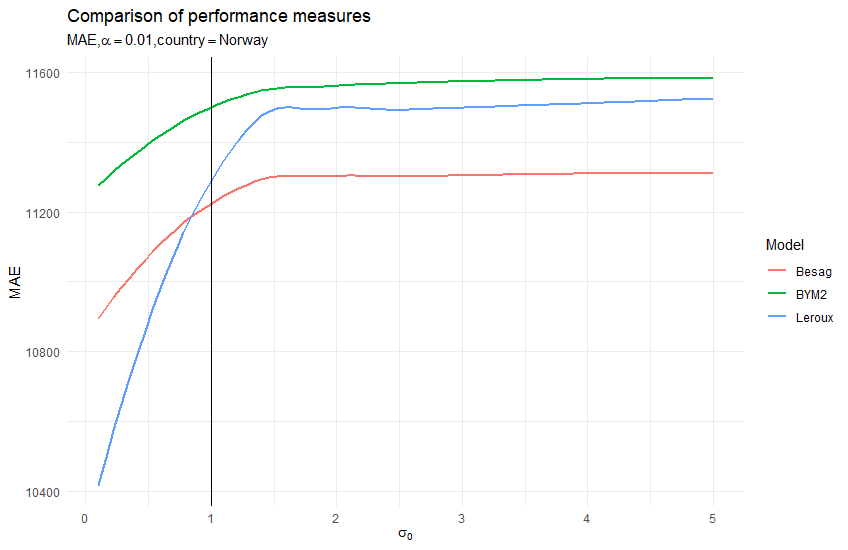
\includegraphics[width = \textwidth]{mae_norway_smooth.png}
    \caption{Value of the MAE when changing the value for $\sigma_0$. The black line highlights the values for $\sigma_0$ = 1.}
    \label{comparison_norway_2}
\end{figure}
% \begin{figure}[H]
%     \centering
%     \includesvg[width = \textwidth]{mae_norway_smooth.svg}
%     \caption{Value of the MAE when changing the value for $\sigma_0$. The black line highlights the values for $\sigma_0$ = 1.}
%     \label{comparison_norway_2}
% \end{figure}
By allowing the precision to be greater, the variance is forced to be smaller. Hence, choosing a lower value for the precision leads to lower values for the WAIC. While this indicates a better fit to the training data, Figure~\ref{comparison_norway_2} also shows that the MAE increases when a higher value for $\sigma_0$ is chosen, as the models overfit on the training data and therefore make worse predictions. \\
The corresponding figures for Germany are shown in Figure~\ref{comparison_germany_1} and Figure~\ref{comparison_germany_2} in the Appendix. \\
Figure~\ref{comparison_norway_5} shows how the credibility intervals of the coefficients of a BYM2 model change when the value for $\sigma_0$ is increased. In general, the credibility intervals for $\sigma_0 = 1$ are narrower than those for $\sigma_0 = 0.1$, but no significant changes are seen between $\sigma_0 = 1$ and $\sigma_0 = 5$. The values of the coefficients tend to remain relatively similar most of the time, especially when the value of the coefficient is close to 1. However, a few times, for example for the variables immigrants\_total, platform and unemp\_immg, the values differ. Furthermore, the coefficients for $\sigma_0 = 1$ and $\sigma_0 = 5$ are more closer to 1 than the ones for $\sigma_0=0.1$ The reason for that is that a higher value for $\sigma_0$ makes the variance of the spatial field larger, therefore the posterior mean should shrink towards 1.
\begin{figure}[H]
    \centering
    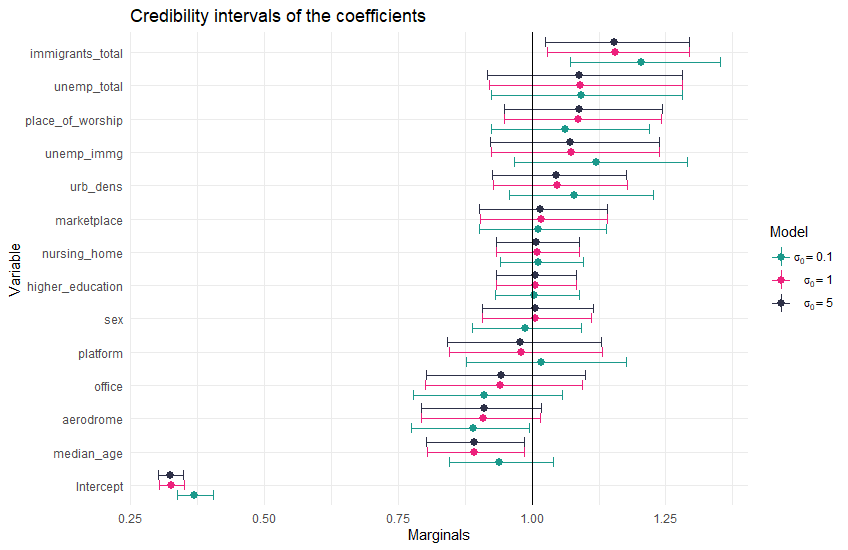
\includegraphics[width = \textwidth]{intervals_prior_norway.png}
    \caption{Comparison of the credibility intervals of a BYM2 model for different values of $\sigma_0$.}
    \label{comparison_norway_5}
\end{figure}
% \begin{figure}[H]
%     \centering
%     \includesvg[width = \textwidth]{intervals_prior_norway.svg}
%    \caption{Comparison of the credibility intervals of a BYM2 model for different values of $\sigma_0$.}
%     \label{comparison_norway_5}
% \end{figure}
The corresponding figure for Germany is shown in Figure~\ref{comparison_germany_5} in the Appendix. \\
Figure~\ref{comparison_norway_6} and Figure~\ref{comparison_norway_7} underline the problem of the models not being comparable with each other. Figure~\ref{comparison_norway_6} already shows slight differences in the spatial field of the Besag Model and the Leroux Model, e.g. in the central and northern parts of Norway, where the posterior mean is higher for the Leroux Model. However, the problem becomes clear when comparing the spatial fields of the Besag model and the Leroux model with the spatial fields of the BYM2 model shown in Figure~\ref{comparison_norway_7}. In the left part of the figure~\ref{comparison_norway_7} the values of the equation~\ref{eq:bym2_1} are plotted, while in the right part the values of $u_{*}$ are plotted. \\
For the spatial field of the unstructured random effect, the values of the posterior mean are similar to the values of the Besag model. For the structured component, however, there are more extreme values, with the posterior mean for northern Norway mostly around -2 and the posterior mean around the Oslo region around 1.5. For comparison, these values are around -1 and 0.8 for the Besag model and -0.8 and 0.6 for the Leroux model, respectively.
\begin{figure}[H]
    \centering
    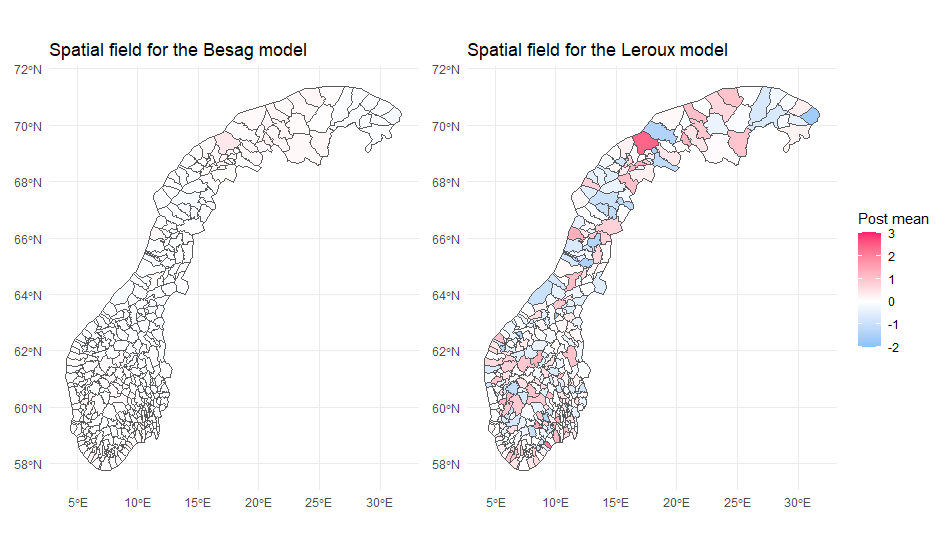
\includegraphics[width = \textwidth]{spatial_field_norway_1.png}
    \caption{Spatial field for a Besag model and a Leroux model.}
    \label{comparison_norway_6}
\end{figure}
% \begin{figure}[H]
%     \centering
%     \includesvg[width = \textwidth]{spatial_field_norway_1.svg}
%    \caption{Spatial field for a Besag model and a Leroux model.}
%     \label{comparison_norway_6}
% \end{figure}
\begin{figure}[H]
    \centering
    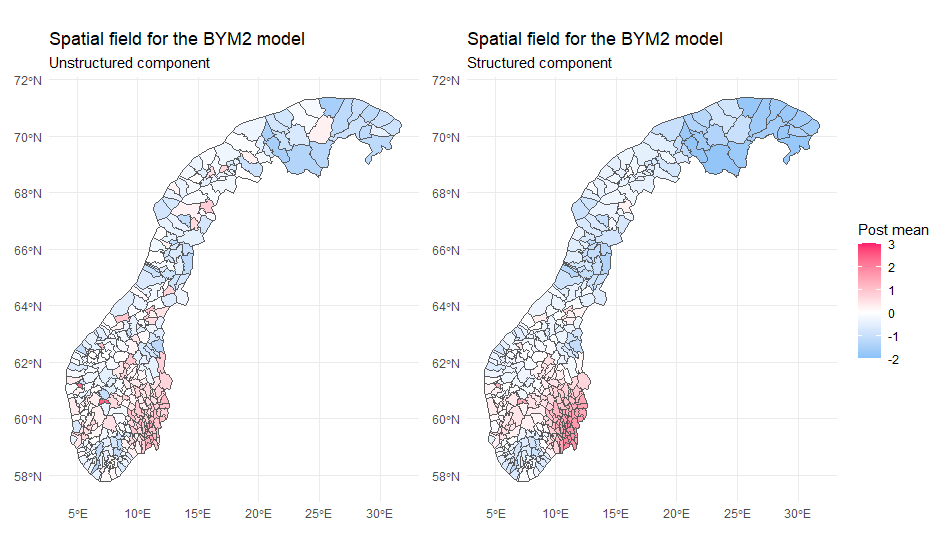
\includegraphics[width = \textwidth]{spatial_field_norway_2.png}
    \caption{Spatial fields for a BYM2 model.}
    \label{comparison_norway_7}
\end{figure}
% \begin{figure}[H]
%     \centering
%     \includesvg[width = \textwidth]{spatial_field_norway_2.svg}
%    \caption{Spatial fields for a BYM2 model.}
%     \label{comparison_norway_7}
% \end{figure}
Finally, looking at the spatial field of the structured component when changing the value for $\sigma_0$, as seen in Figure~\ref{comparison_norway_8}, it can be seen that for a small value like $\sigma_0 = 0.1$, the values of the posterior mean are mostly around 0, while for a higher value not much change can be seen. Interestingly, however, if the posterior mean is given its own scale for $\sigma_0 = 0.1$, as done in Figure~\ref{comparison_norway_9}, it can be seen that the higher up north a municipality lies, the lower the posterior mean becomes. The reason for this is that if $\sigma_0$ is small, the spatial field is only one plane. $\sigma_0$ specifies how much the spatial effect is allowed to deviate from this plane, and with a small value for $\sigma_0$ only a small deviation is allowed, which can then look similar to a linear effect.
\begin{figure}[H]
    \centering
    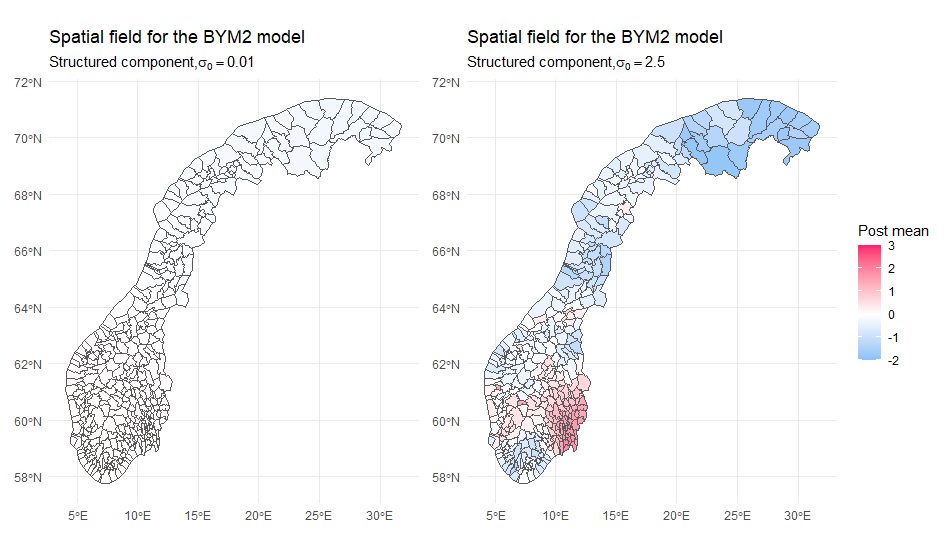
\includegraphics[width = \textwidth]{spatial_field_norway_3.png}
    \caption{Spatial fields for the structured component of a BYM2 model when changing the value for $\sigma_0$.}
    \label{comparison_norway_8}
\end{figure}
% \begin{figure}[H]
%     \centering
%     \includesvg[width = \textwidth]{spatial_field_norway_3.svg}
%    \caption{Spatial fields for the structured component of a BYM2 model when changing the value for $\sigma_0$.}
%     \label{comparison_norway_8}
% \end{figure}
\begin{figure}[H]
    \centering
    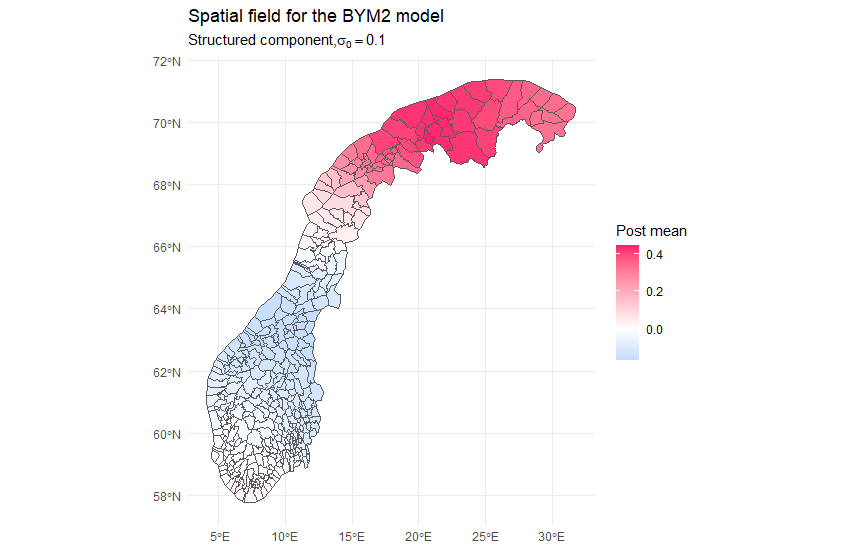
\includegraphics[width = \textwidth]{spatial_field_norway_4.png}
    \caption{Structured component of the spatial field for a BYM2 model.}
    \label{comparison_norway_9}
\end{figure}
% \begin{figure}[H]
%     \centering
%     \includesvg[width = \textwidth]{spatial_field_norway_4.svg}
%    \caption{Structured component of the spatial field for a BYM2 model.}
%     \label{comparison_norway_9}
% \end{figure}
The corresponding figures for Germany are shown in Figure~\ref{comparison_germany_6}, Figure~\ref{comparison_germany_7}, Figure~\ref{comparison_germany_8} and Figure~\ref{comparison_germany_9} in the Appendix. \\
\clearpage
\section{Spatio-Temporal Models}
\subsection{Spatio-Temporal Models for Germany}
\subsection{Spatio-Temporal Models for Norway}
\clearpage
\section{Predictive Models}
\subsection{Predictive Models for Germany}
\subsection{Predictive Models for Norway}